\begin{comment}
  \bibliography{project.bib}
\end{comment}

\chapter{Digital Image}
\label{cha:digital-image}

\section{Color}
\label{sec:color}

\subsection{What is color?}
\label{sec:what-color}

\newcommand{\bluewave}{\ensuremath{\SI{400}{\nano\meter}}}

Color is light. Light on the other hand, is composed of tiny particles
traveling at different wavelengths. \cite{neider93:_openg_progr_guide}
So light is just a wave. Figure \ref{fig:wave} demonstrates what a
wave looks like and what a wavelength measures. Different colors have
different wavelengths. For example: blue, as shown in figure
\ref{fig:wave}, has a wavelength of
\bluewave. \cite{ohlsson99:_digit_bild_kreat} That's $0.00000004$
meters!

\begin{figure}[h!]
  \centering
  \inputtikz{wave.tex}
  \caption{A blue lightwave. $\lambda$ is the letter commonly used to
    represent  wavelength.}
  \label{fig:wave}
\end{figure}

But how do our eyes see these light waves? In our eyes, there are
cells for perceiving three different kinds of wavelengths of light:
red, blue and green. When these cells absorb light, we see color. And
when these cells absorb mixed amounts and/or different amounts of red,
blue and green light, we are able to perceive \textit{all} the other
possible colors.

\subsection{RGB}
\label{sec:rgb}

Color models are ways specifying color numerically \todo{mention
  additive and subtractive color models here}
\cite{fadgi11:color_model}. They are of course very convenient for
computer since they are very good at dealing with numbers. A very
widely used color model for representing color in computer is
\textbf{RGB} \index{RGB}.

\begin{figure}[h]
  \centering
  \inputtikz{rgb.tex}
  \caption{RGB color model}
  \label{fig:rgb}
\end{figure}

The color model is, of course, based on how our eyes perceive color, as
mentioned in section \ref{set:what-color}. Do, however, observe figure
\ref{fig:rgb}. As it can be seen, all the other colors can be achieved
by mixing red, blue and green. Also note that white is achieved by
mixing all of three colors. And black is represented by no light at
all. One last thing: The different values for red, blue and green are
their channels.

\subsection{CMYK}
\label{sec:cmyk}

\subsection{Alpha channel}
\label{sec:alpha_chan}

But there is actually even more to RGB. There is an extended color
model of RGB that's called RGBA \index{RGBA}(it is sometimes also
referred to as ARGB \index{ARGB}). In this model a new channel is
added: the alpha channel \index{alpha channel}. This new channel
represents the opacity of a color. Opacity is simply the opposite of
transparency. Thus, a low transparency means that the color in
question is close to invisible  \cite{porter84_compos_dig_img}.

\section{Color depth}
\label{sec:color-depth}

\newcommand{\rgbtrip}[3]{( \textcolor{red}{#1},\textcolor{green}{#2},\textcolor{blue}{#3})}

But up until now, we have said nothing about how the computer
represents these color model. Let us start with:

\subsection{24-bit color}
\label{sec:24-bit-color}

So each color is just a combination red,blue and green lights. In the
RGB color model these channels are given values. Let us represent
these values as a triple of three numbers, like this:
\rgbtrip{123}{21}{91}.

An 8-bit number has ,as familiar, only $255$ possible values. If we
assign an  8-bit number to each color channel, the color's total size
will be 24-bits. This way of representing color is called 24-bit color
\index{24-bit color}. You can also say that its color depth \index{color
  depth} is 24 bits.

A full red color is represented by the triple \rgbtrip{255}{0}{0}. In
that case, have a guess at what color is represented by
\rgbtrip{255}{0}{255}. If haven't guessed it already, please study
figure \ref{fig:rgb}. As you probably already have guessed, this color
is yellow. And in the same number mixing and matching way, many other
colors can be represented. Like it is represented in color table
\ref{tab:color-examples}

\newcommand{\colorrow}[4]{  \rgbtrip{#1}{#2}{#3} &
  \textcolor[RGB]{#1,#2,#3}{#4} \\ \hline}

\begin{table}[h!]
  \centering
  \begin{tabular}[h!]{|l|l|}
    \hline
    RGB triple & Resulting color \\ \hline
    \colorrow{255}{215}{0}{Gold}
    \colorrow{165}{42}{42}{Brown}
    \colorrow{255}{0}{255}{Purple}
    \colorrow{255}{192}{203}{Pink}
    \colorrow{255}{165}{0}{Orange}
  \end{tabular}
  \caption{Colors}
  \label{tab:color-examples}
\end{table}

But of course, not all colors can be represented using just
24-bit. The number of All possible colors is infinite. But you can
represent an awful not colors with only 24-bits. How many? Well, every
color channel can have $256$ different values. There are $3$
channels. Hence, there are $256^3 = 16777216$ different colors.

\begin{figure}[h!]
  \centering
  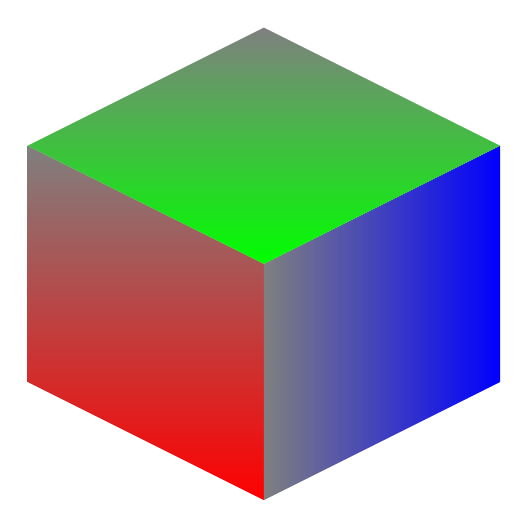
\begin{tikzpicture}
    \shade[yslant=-0.5,bottom color=red]
    (0,0) rectangle +(3,3);

    \shade[yslant=0.5,right color=blue]
    (3,-3) rectangle +(3,3);

    \shade[yslant=0.5,xslant=-1,bottom color=green] (6,3) rectangle +(-3,-3);

  \end{tikzpicture}
  \caption{RGB color cube TODO: Make.}
  \label{fig:color-cube}
\end{figure}

\newcommand{\rgbaquad}[4]{(
  \textcolor{red}{#1},\textcolor{green}{#2},\textcolor{blue}{#3},\textcolor{grey}{#4} )}

Adding alpha channels to this color representation is trivial, just
add a fourth channel. Here is for example the color green halfly
transparent: \rgbaquad{0}{0}{255}{125}. The only real difference is
that a color will require 32-bits of storage if an alpha channel is needed.

\subsection{Other colors depths}
\label{sec:other-colors-depths}

\subsection{Indexed Color}
\label{sec:indexed-color}

% 8-bit color 1-bit color, palettes need to be covered.-

\printbibliography[heading=subbibliography]
